\documentclass[UTF8]{ctexart}
\CTEXsetup[format={\Large\bfseries}]{section}
\usepackage{amsmath}
\usepackage{ctex}
\usepackage{array}
\usepackage{ulem}
\usepackage{graphicx}
\usepackage{geometry}
\usepackage{multirow}
\usepackage{subfig}
\usepackage{float}
\usepackage{multicol}
\usepackage{multirow}
\usepackage{indentfirst}
\usepackage{makecell}
\geometry{papersize={21cm,29.7cm}}
\geometry{left=2.54cm,right=2.54cm,top=3.18cm,bottom=3.18cm}
\usepackage{fancyhdr}
\pagestyle{fancy}
\lhead{\today}
\chead{}
\rhead{2020011075}
\lfoot{清华大学}
\cfoot{\thepage}
\rfoot{物理实验B(2)}
\renewcommand{\headrulewidth}{0.4pt}
\renewcommand{\headwidth}{\textwidth}
\renewcommand{\footrulewidth}{0pt}
\usepackage{bm}
\begin{document}
\begin{titlepage}
    \begin{center}
		\quad \\
		\quad \\
        \quad \\
        \quad \\
        \quad \\
        \quad \\
		\kaishu \fontsize{30}{15} 霍尔效应实验及磁阻测量
	\end{center}
	\vskip 10cm

    \begin{center}
        \begin{large}
        \begin{tabular}{cc}
        院\qquad 系:& ~~~~~~~~自动化系~~~~~~~~      \\
        \cline{2-2}\\
        班\qquad 级:& 自02班   \\
        \cline{2-2}\\
        学生姓名:& 彭程    \\
        \cline{2-2}\\
        学\qquad 号:&2020011075   \\
        \cline{2-2}\\
        组\qquad 号:& 双四下L    \\
        \cline{2-2}\\
        座~~位~~号:& \# 5    \\
        \cline{2-2}
        \end{tabular}
        \end{large}
        \end{center}

\end{titlepage}
\newpage
\tableofcontents
\newpage
\section{实验名称}
霍尔效应实验及磁阻测量
\section{实验目的}
\begin{enumerate}
\item 了解霍尔效应的产生原理以及副效应的产生原理;
\item 掌握霍尔系数的测量方法,学习消除霍尔副效应的实验方法;
\item 研究半导体材料的电阻值随磁场的变化规律。
\end{enumerate}
\section{实验原理}
    \subsection {霍尔效应} 
    如下图所示为霍尔效应产生的模型简化与简要分析:

    \begin{figure}[H]
        \centering
        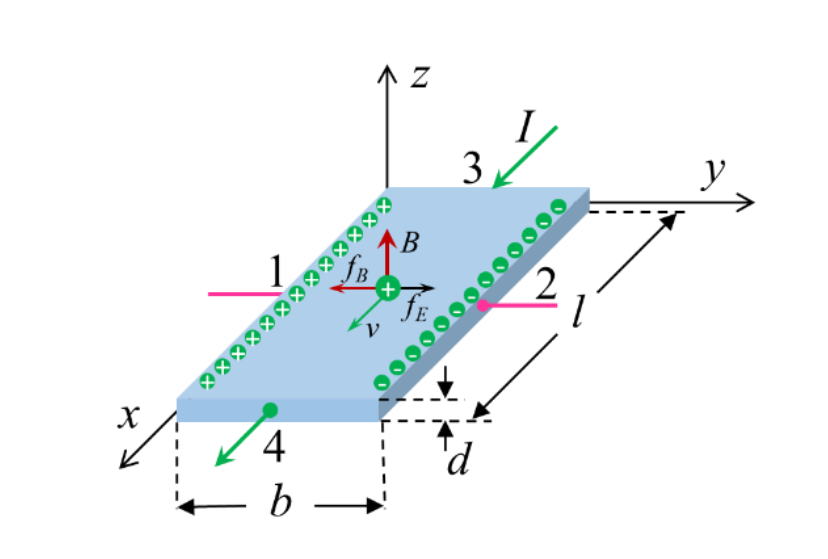
\includegraphics[scale=0.5]{霍尔原理.png}
        \caption{霍尔效应模型}
        \label{fig:label}
    \end{figure}
    

    在如图所示的位置加上磁场后,在载流子收到的洛伦兹力和电场力达到平衡时,1、2 点间产生电位差。这个电位差与电流强度I 及磁感应强度B 均成正比,与板的厚度d 成反比,即
    $$
    U_H = R_H\frac{IB}{d} = K_HIB
    $$

    其中$U_H$为霍尔电压,$R_H$为霍尔系数,$K_H = R_H / d$为霍尔片的灵敏度。

    而洛伦兹力和电场力达到平衡状态时有$f_B = f_E$,即$evB = eE = eU_H /b$。
    
    于是1、2 两点间的电位差为: 
    $$
    U_H = vbB \nonumber 
    $$

    而电流为:
    $$
    I = nevbd \nonumber 
    $$

    所以有:
    $$  
    U_H = \frac{IB}{ned}
    $$

    可以得到霍尔系数及霍尔片的灵敏度为:

    \begin{align}
        R_H = \frac{1}{ne} \nonumber  \\
        K_H = \frac{R_H}{d} \nonumber 
    \end{align}

    \subsection {霍尔效应的副效应} 

    除霍尔效应外,还有一些副效应与霍尔效应一同发生,会导致霍尔电压的测量产生误差,因此应当在实验过程中尽量消除这些效应的影响。

   1. 厄廷好森(Etinghausen)效应引起的电位差$U_E$
  
   2. 能斯脱(Nernst)效应引起的电位差$U_N$

   3. 里纪-勒杜克(Righi-Leduc)效应引起的电位差$U_R$
   
   4. 不等位效应引起的电位差$U_0$

   5. 附加电压$U_S$

    当I、B 确定后,霍尔片的输出电压为上述几项的代数和:
    $$
    U = f(U_H, U_E, U_N, U_R, U_0, U_S)
    $$

    通过改变工作电流I 的方向和外加磁场B 的方向的不同组合测量可以消除或减少$U_N$、$U_R$ 和$U_0$ 的影响。重点是消除不等位效应$U_0$。
   





    \subsection {磁电阻效应原理} 

    设磁阻器件在零磁场时电阻及电阻率分别为$R(0)$,$\rho(0)$,磁场为B 时电阻及电阻率分别为R(B),$\rho(B)$。
    一般正常磁阻器件的$\Delta R/R(\theta)$ 在弱磁场条件下正比于$B^2$,而强磁场条件下$\Delta R/R(\theta)$ 则正比于$B$。对于实验所用器件,$B \leq 0.06T$ 可看作弱磁场条件,$B \geq 0.12T $可看作强磁场条件。
 


\section{实验仪器}
\begin{enumerate}
  \item 万用表
  \item 霍尔元件磁阻元件及电磁铁 (仪器编号:110832)
  \item 电流源
\end{enumerate}

\noindent 相关参数:

     励磁电流: $I_M$ = 0 $\sim$ 1000mA
     
     工作电流: $I_S$ = 1.5 $\sim$ 10mA

     霍尔片尺寸: 300 $\times$ 100 $\times$ 3µm

     当 $I_M = 500mA$ 时,磁极中心磁感应强度$ B = 131.4mT$

\section{实验步骤}
\begin{enumerate}
  \item 设计电路,画出完整电路图;
  \item 测量霍尔片输出电压$U_H$ 与输入电流I 的关系曲线,计算有关的霍尔片参数;
  \item 判断霍尔片的载流子类型;
  \item 标定激励电流$I_M(0 \sim 800mA)$ 与磁极间磁场B 的关系;
  \item 测定磁极间隙水平方向磁场的分布曲线B $\sim$ x;
  \item 测量霍尔片中载流子的迁移率$\mu$;
  \item 研究锑化铟磁阻器件的磁电阻效应
\end{enumerate}

\section{数据处理}

霍尔效应实验电路设计如下:

\begin{figure}[H]
  \centering
  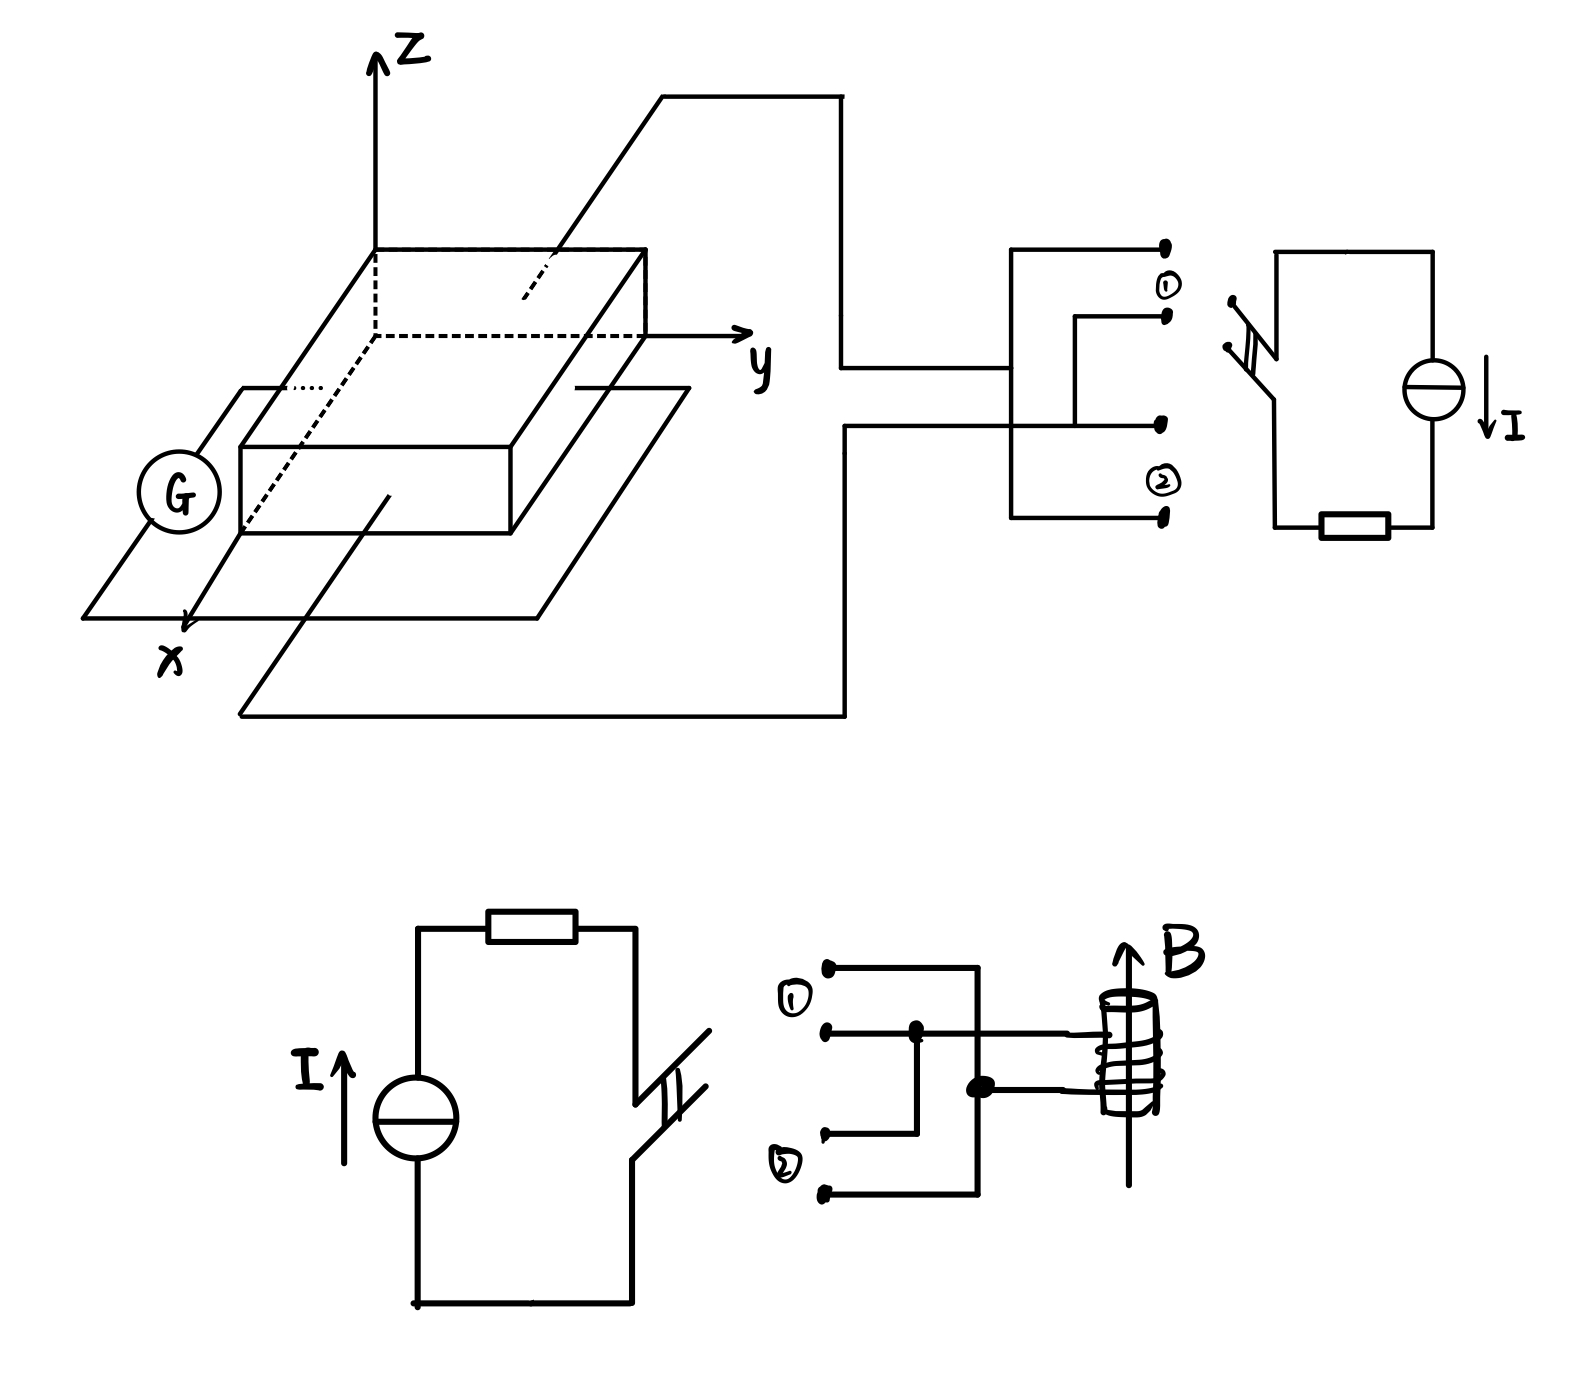
\includegraphics[scale=0.15]{电路.jpg}
  \caption{霍尔效应实验电路图} %最终文档中希望显示的图片标题
\end{figure}



\subsection{测量霍尔片输出电压 $U_H$ 与输入电流$I$ 的关系曲线}

实验中测量数据整理如下表所示:

\begin{center}
\begin{tabular}{c|c|c|c|c|c}
  \hline I(mA) & $U_1(mV)$ & $U_2(mV)$ & $U_3(mV) $ & $U_4(mV)$ &$U_H(mV)$ \\
  \hline 2.00  & -46.1  & 46.0  & -45.7  & 45.7  & -45.88       \\
  \hline 3.00  & -68.9  & 68.8  & -68.4  & 68.4  & -68.63       \\
  \hline 4.00  & -91.7  & 91.6  & -91.1  & 91.0  & -91.35       \\
  \hline 5.00  & -114.5  & 114.2  & -113.7  & 113.6  & -114.00  \\
  \hline 6.00  & -137.5  & 137.1  & -136.5  & 136.3  & -136.85  \\
  \hline 7.00  & -160.6  & 160.0  & -159.4  & 159.0  & -159.75  \\
  \hline 7.30  & -183.5  & 182.5  & -182.1  & 181.6  & -182.43  \\
  \hline
\end{tabular}\\
\end{center}

对上述数据进行线性拟合,得到关系曲线及拟合关系如下所示:
\begin{figure}[H]
  \centering
  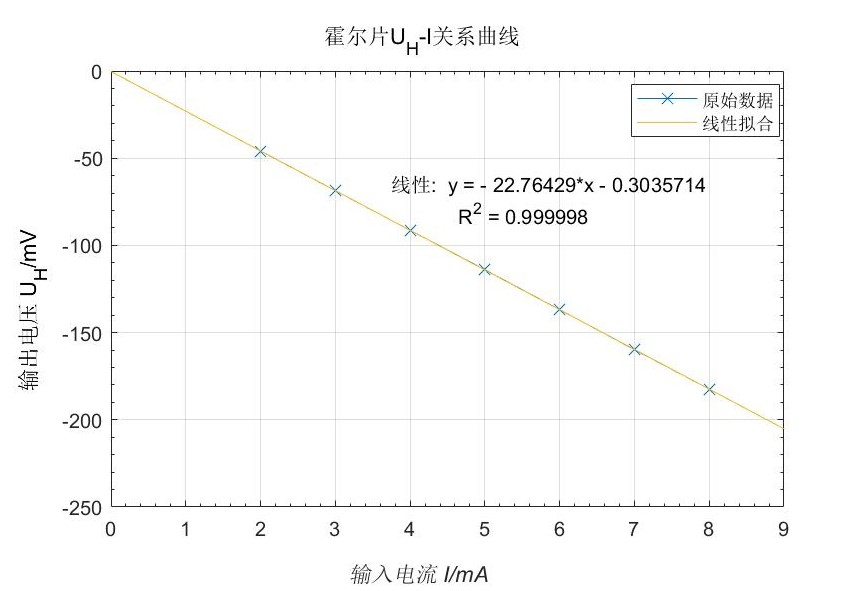
\includegraphics[scale=0.7]{拟合1.jpg}
\end{figure}

根据线性拟合关系,相关系数 $R^2$ = 0.999998,表明线性相关系数强,拟合直线斜率 $k \approx -22.76(V/A)$。

由此计算霍尔片灵敏度:

$$
K_H = \frac{U_H}{IB}= \frac{k}{B} = \frac{-22.76}{131.4\times10^{-3}} = -173.21~\Omega/T
$$

霍尔系数为:

$$
R_H = K_H \cdot d = 173.21\times 3 \times10^{-6} = -5.1963\times10^{-4}\Omega\cdot m/T
$$

载流子浓度为:

$$
n = \frac{1}{R_He} = \frac{1}{5.1963\times10^{-4}\times 1.602\times10^{-19}} = 1.2013\times10^{22}~m^{-3}
$$

计算拟合斜率不确定度:
$$
s_{k}=t_{p}(n-2)|k| \sqrt{\frac{r^{-2}-1}{n-2}}=2.57 \times 22.76 \times \sqrt{\frac{0.999998^{-2}-1}{7-2}}=0.052 \mathrm{~V} / \mathrm{A}
$$

计算  $K_{H} $ 不确定度:
$$
\Delta K_{H}=\frac{1}{B_{0}} s_{k}=\frac{0.052}{131.4 \times 10^{-3}}=0.40 V /(A \cdot T)$$

计算  $R_{H}$  不确定度:
$$
\Delta R_{H}=\Delta K_{H} d=0.395 \times 3 \times 10^{-6}=1.2 \times 10^{-6} \mathrm{~m}^{3} / C
$$

计算载流子浓度  $n $ 不确定度:
$$
\Delta n=\sqrt{\left(\frac{\partial n}{\partial R_{H}}\right)^{2}\left(\Delta R_{H}\right)^{2}}=n \frac{\Delta R_{H}}{R_{H}}=1.2013 \times 10^{22} \times \frac{1.18 \times 10^{-6}}{5.1936 \times 10^{-4}}=2.7 \times 10^{19} \mathrm{~m}^{-3}
$$

由计算结果可得各物理量的最终结果为:
\begin{center}
  霍尔片灵敏度 $K_{H}=(-173.21 \pm 0.40) V /(A \cdot T)$
\end{center}
\begin{center}
  霍尔系数$R_{H}=(-5.196 \pm 0.012) \times 10^{-4} m^{3} / C$
\end{center}
\begin{center}
  载流子浓度$n=(1.2013 \pm 0.0027) \times 10^{22} m^{-3}$
\end{center}

\noindent \textbf{该实验部分的思考题:如何测量不等位电压?}

\noindent 解答:

由于制作工艺限制,  1 、 2  两点不处于同一等位线上, 因此在磁场  B  不存在时,  1 、 2  两点间也存在电 位差  $U_{0}$ , 此即不等位效应。若需观测不等位效应, 可设置励磁电流  $I_{M}=0 $, 记录该工作条件下的霍尔电压  $U_{H}$ , 即为该工作电流 下对应的不等位电压。

\subsection{判断霍尔片的载流子类型}

\begin{figure}[H]
  \centering
  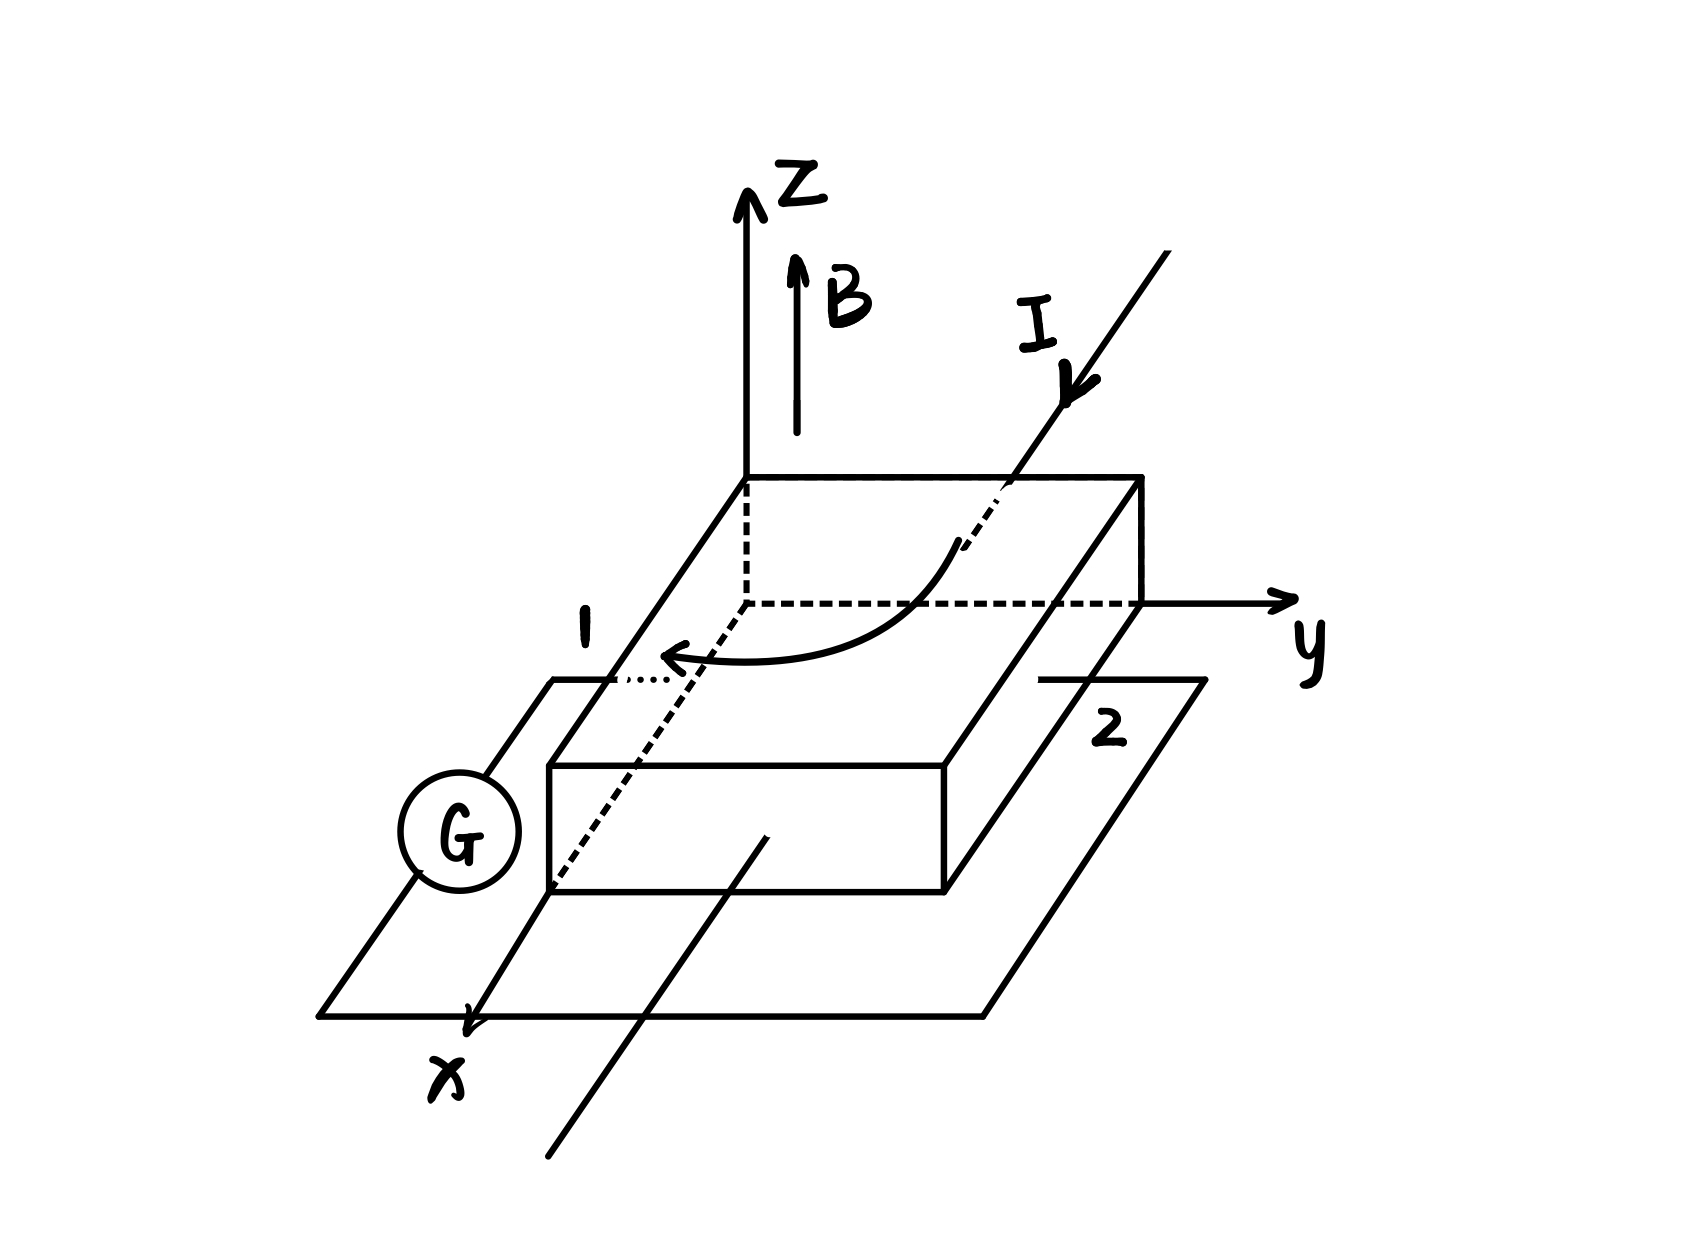
\includegraphics[scale=0.15]{载流子类型.jpg}
  \caption{载流子类型示意图} %最终文档中希望显示的图片标题
\end{figure}


霍尔片载流子应为电子,霍尔片材质为 N 型半导体。

如上图所示,当测量值为$U_1$时,即+B+I时,测得 $U_H$ < 0。根据左手定则判断此时载流子应当在1处聚集,而这样导致1处电位低于2处,说明载流子为电子,即霍尔片材质为N型半导体。


\subsection{标定激励电流$I_M$与磁极间磁场B 的关系}

\begin{center}
\begin{tabular}{c|c|c|c|c|c|c}
  \hline $I_M/mA$ & $U_1/mV$ & $U_2/mV$ & $U_3/mV $ & $U_4/mV$ &$U_H(mV)$ & B(mT) \\
  \hline 100   & -18.9  & 18.6  & -18.1  & 18.0  & -18.4  & 26.6  \\
  \hline  200   & -37.1  & 37.0  & -36.5  & 36.4  & -36.8  & 53.0  \\
  \hline  300   & -55.6  & 55.3  & -54.8  & 54.7  & -55.1  & 79.5  \\
  \hline  400   & -74.0  & 73.6  & -73.1  & 73.0  & -73.4  & 106.0  \\
  \hline  500 & -91.8  & 91.7  & -91.2  & 91.2  & -91.5  & 132.0  \\
  \hline  600 & -109.9 & 109.8 & -109.2  & 109.3 & -109.6 & 158.1 \\
  \hline  700 & -127.9 & 127.8 & -127.2  & 127.2 & -127.5 & 184.1 \\
  \hline  800 & -145.6 & 145.6 & -145.0  & 145.1 & -145.3 & 209.8  \\
  \hline  900 & -162.8 & 162.8  & -162.1  & 162.3 & -162.5 & 234.5 \\
  \hline 1000& -179.9 & 179.9  & -179.2  & 179.4 & -179.6 & 259.2  \\
  \hline
\end{tabular}\\
\end{center}

其中, $ U_{H}$ 、$ B $ 的计算公式分别为:

$$
\begin{array}{c}
U_{H}=\frac{1}{4} \times\left(U_{1}-U_{2}+U_{3}-U_{4}\right) \\
B=\frac{U_{H}}{K_{H} I}=\frac{U_{H}}{-173.21 \times 4 \times 10^{-3}}
\end{array}
$$

对上述数据进行线性拟合,得到关系曲线及拟合关系如下所示:
\begin{figure}[H]
  \centering
  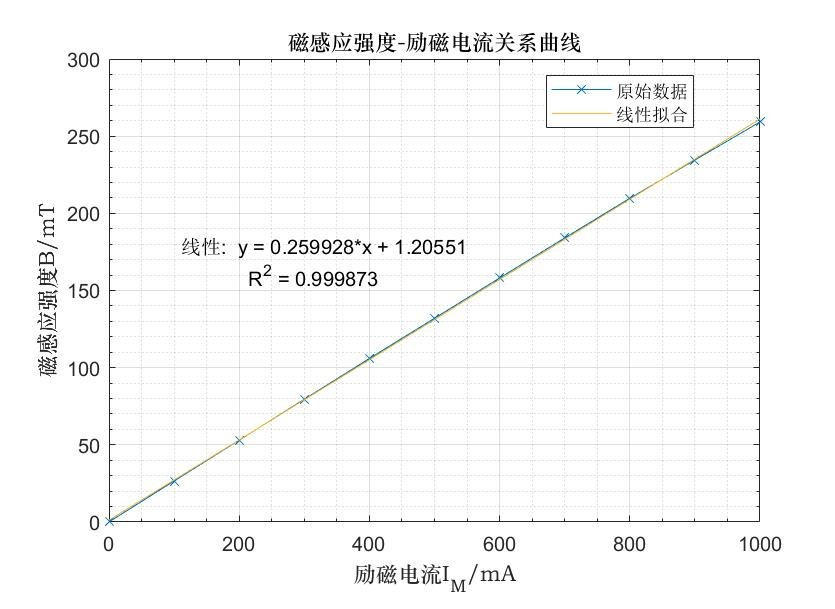
\includegraphics[scale=0.6]{拟合2.jpg}
\end{figure}

线性拟合所得直线为 $ B=0.2599 I_{M}+1.2055$ , 相关系数 $ R^{2}=0.9999987$ , 表明线性相关系数强, 与理论分析相符。


\subsection{测定磁极间隙水平方向磁场的分布曲线B $\sim$ x}

实验测量结果如下表所示 ($I_S = 4.00mA$, $I_M = 500mA$)。

\begin{center}
  
  \begin{tabular}{c|c|c|c|c|c|c}
    \hline $x/mm$ & $U_1/mV$ & $U_2/mV$ & $U_3/mV $ & $U_4/mV$ &$U_H(mV)$ & $B(mT)$ \\
    \hline
    0.0   & -23.8 & 23.6  & -23.2 & 23.0  & -23.4 & 33.8 \\
    \hline
    4.0   & -28.9 & 28.7  & -28.3 & 28.1  & -28.5 & 41.1 \\
    \hline
    6.0   & -33.6 & 33.4  & -33.0 & 32.8  & -33.2 & 47.9 \\
    \hline
    8.0   & -41.4 & 41.2  & -40.7 & 40.6  & -41.0 & 59.1 \\
    \hline
    10.0  & -54.3 & 54.2  & -53.7 & 53.6  & -54.0 & 77.9 \\
    \hline
    12.0  & -69.9 & 69.9  & -69.4 & 69.4  & -69.7 & 100.5 \\
    \hline
    14.0  & -85.1 & 85.0  & -84.5 & 84.5  & -84.8 & 122.4 \\
    \hline
    16.0  & -89.3 & 89.2  & -88.7 & 88.7  & -89.0 & 128.4 \\
    \hline
    18.0  & -90.8 & 90.7  & -90.2 & 90.1  & -90.5 & 130.5 \\
    \hline
    20.0  & -91.0 & 90.9  & -90.4 & 90.4  & -90.7 & 130.9 \\
    \hline
    25.0  & -91.2 & 91.1  & -90.6 & 90.5  & -90.9 & 131.1 \\
    \hline
    30.0  & -91.3 & 91.2  & -90.7 & 90.7  & -91.0 & 131.3 \\
    \hline
    40.0  & -91.6 & 91.5  & -91.0 & 90.9  & -91.3 & 131.7 \\
    \hline
    45.0  & -91.7 & 91.6  & -91.1 & 91.0  & -91.4 & 131.8 \\
    \hline
    47.0  & -91.6 & 91.4  & -90.9 & 90.9  & -91.2 & 131.6 \\
    \hline
    49.0  & -90.4 & 90.3  & -89.8 & 89.8  & -90.1 & 130.0 \\
    \hline
    51.0  & -85.5 & 85.4  & -84.9 & 84.8  & -85.2 & 122.9 \\
    \hline
    53.0  & -73.3 & 73.3  & -72.8 & 72.6  & -73.0 & 105.4 \\
    \hline
    55.0  & -55.5 & 55.3  & -54.8 & 54.6  & -55.1 & 79.5 \\
    \hline
    57.0  & -42.1 & 42.0  & -41.5 & 41.4  & -41.8 & 60.3 \\
    \hline
    59.0  & -34.6 & 34.4  & -34.0 & 33.8  & -34.2 & 49.4 \\
    \hline
    60.0  & -31.7 & 31.5  & -31.1 & 30.9  & -31.3 & 45.2 \\
    \hline
  \end{tabular}%
\end{center}

其中, $ U_{H}$ 、$ B $ 的计算公式分别为:

$$
\begin{array}{c}
U_{H}=\frac{1}{4} \times\left(U_{1}-U_{2}+U_{3}-U_{4}\right) \\
B=\frac{U_{H}}{K_{H} I}=\frac{U_{H}}{-173.21 \times 4 \times 10^{-3}}
\end{array}
$$

根据上表,作出磁感应强度与水平磁隙 $B \sim x$ 关系图线如下图所示:

\begin{figure}[H]
  \centering
  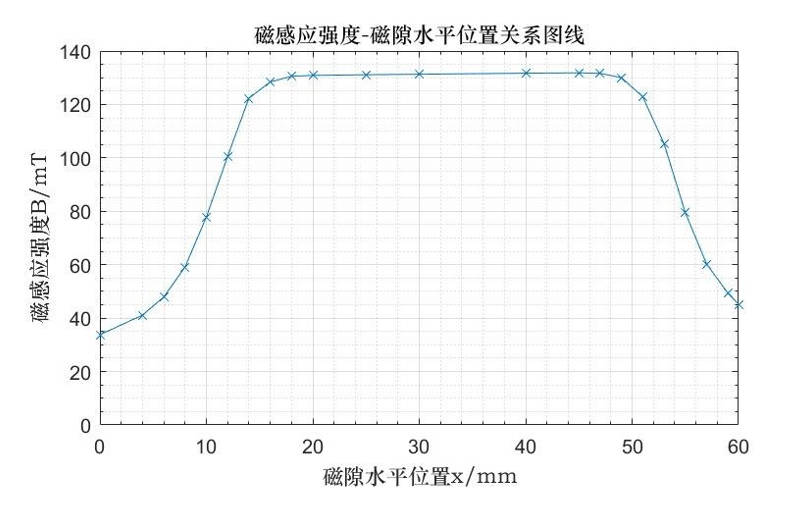
\includegraphics[scale=0.5]{拟合3.jpg}
\end{figure}

根据图线可得出,在 $18.0mm \leq x \leq 49.0mm $范围内,磁感应强度稳定。计算得均匀磁场区间长度为$31.0mm$。

根据该区域内的磁感应强度取平均值,可得 $\bar{B} = 131.1mT$。

\subsection{测量霍尔片中的载流子迁移率$\mu$}

实验测量结果如下表所示 $ \left(I_{M}=0 m A\right)$  。

\begin{center}
\begin{tabular}{c|c|c|c|c|c|c}
  \hline $I_{S} / m A$  &  2.00  &  3.00  &  4.00  &  5.00  &  6.00  &  7.00   \\
  \hline $U / V$  &  1.481  &  2.236  &  2.991  &  3.761  &  4.550  &  5.365    \\
  \hline
  \end{tabular}
\end{center}

将上表数据进行线性拟合结果如下:
\begin{figure}[H]
  \centering
  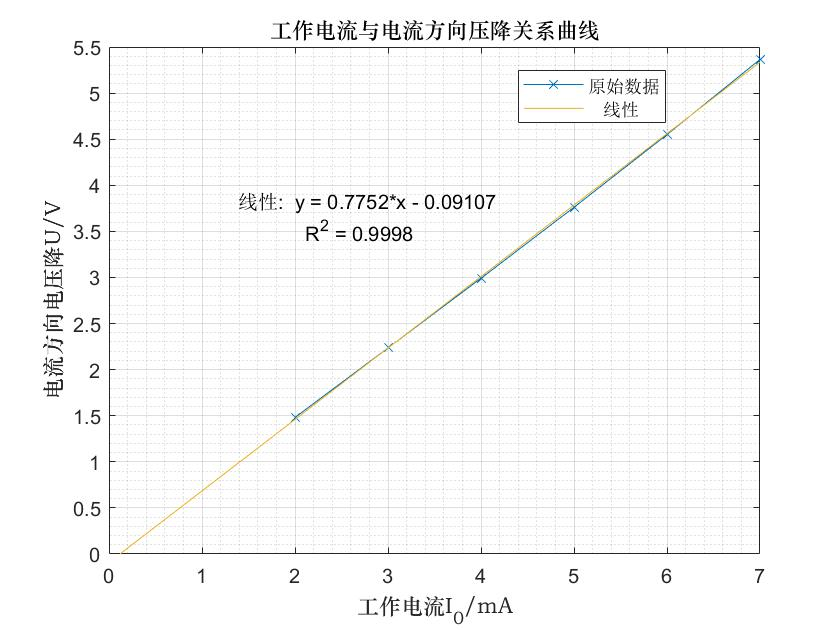
\includegraphics[scale=0.5]{拟合4.jpg}
\end{figure}

将上述测量结果拟合成直线线性拟合所得直线为 $ U=0.7752 I_{s}-0.09107$ , 相关系数 $ R^{2}=0.9998$ , 表明线性相关系数强。

根据上述拟合结果,可以得到:
$$
\frac{U}{I}=k = 0.7752 \times 10^{3} \Omega
$$

而通入电流方向场强:
$$
E=\frac{U}{l}
$$

载流子平均运动速率:
$$
v=\frac{I}{n e S}=\frac{\left|K_{H}\right| I}{b}
$$

所以霍尔元件载流子迁移率$\mu$为:
$$
\mu=\frac{v}{E}=\frac{\left|K_{H}\right| I l}{b U}=\frac{\left|K_{H}\right| l}{bk}=\frac{173.21\times 300 \times 10^{-6}}{100 \times 10^{-6}\times 0.775\times 10^{3}}=0.670 \mathrm{~m}^{2} /(V \cdot s)
$$


\subsection{研究锑化铟磁阻器件的磁电阻效应}

实验测量结果如下表所示 ($I_S = 4.00mA$, $I_M = 500mA$)

\begin{center}
  \begin{tabular}{c|c|c|c|c|c}
    \hline $I_M(mA)$ & $U_{CD}(V)$ & $B(mT)$ & $R(B)(\Omega) $ & $\Delta R(\Omega)$ &$\Delta R/R(0)$ \\
   \hline
    0     & 0.4176 & 1.206  & 278.4000  & 0.00  & 0.0000 \\
   \hline
    50    & 0.4212 & 14.201  & 280.8000  & 2.40  & 0.0086 \\
   \hline
    100   & 0.4303 & 27.196  & 286.8667  & 8.47  & 0.0304 \\
   \hline
    150   & 0.4450 & 40.191  & 296.6667  & 18.27  & 0.0656 \\
   \hline
    200   & 0.4641 & 53.186  & 309.4000  & 31.00  & 0.1114 \\
   \hline
    250   & 0.4847 & 66.181  & 323.1333  & 44.73  & 0.1607 \\
   \hline
    300   & 0.5083 & 79.176  & 338.8667  & 60.47  & 0.2172 \\
   \hline
    350   & 0.5336 & 92.171  & 355.7333  & 77.33  & 0.2778 \\
   \hline
    400   & 0.5582 & 105.166  & 372.1333  & 93.73  & 0.3367 \\
   \hline
    500   & 0.6003 & 131.156  & 400.2000  & 121.80  & 0.4375 \\
   \hline
    600   & 0.6310 & 157.146  & 420.6667  & 142.27  & 0.5110 \\
   \hline
    700   & 0.6550 & 183.136  & 436.6667  & 158.27  & 0.5685 \\
   \hline
    800   & 0.6757 & 209.126  & 450.4667  & 172.07  & 0.6181 \\
   \hline
    900   & 0.6957 & 235.116  & 463.8000  & 185.40  & 0.6659 \\
   \hline
    1000  & 0.7150 & 261.106  & 476.6667  & 198.27  & 0.7122 \\
    \hline
\end{tabular}
\end{center}

其中, $ U_{C D}$  为利用万用表电压档直接测得, 其他数据的计算公式为:
磁感应强度为 $ B$  时, 磁阻器件的等效电阻:
$$
R(B)=\frac{U_{C D}}{I_{C D}}=\frac{U_{C D}}{1.5 \times 10^{-3} A}
$$

 $\Delta R $ 表示上述等效电阻与 $ R(0)$  之差  $\Delta R=R(B)-R(0)$ , 比值表示为 $ \Delta R / R(0)$  。 磁感应强度 $ B $ 根据  6.3  中拟合所得直线计算得出:
$$
B=0.2599 I_{M}+1.2055
$$

作出磁感应强度与电阻比值  $\frac{\Delta R}{R(0)} \sim B  $关系图线如下图所示:

\begin{figure}[H]
  \centering
  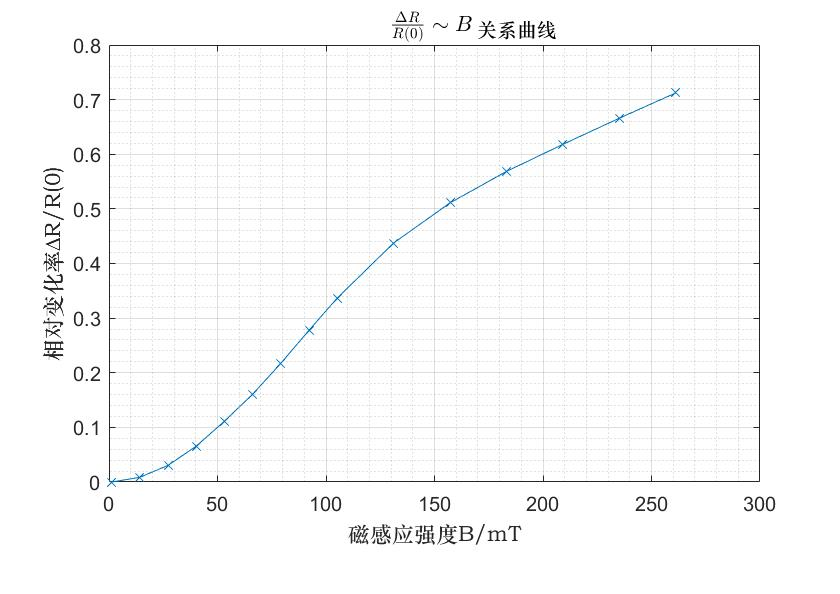
\includegraphics[scale=0.5]{拟合5.jpg}
\end{figure}

\begin{figure}[htbp]
	\centering
	\begin{minipage}{0.49\linewidth}
		\centering
		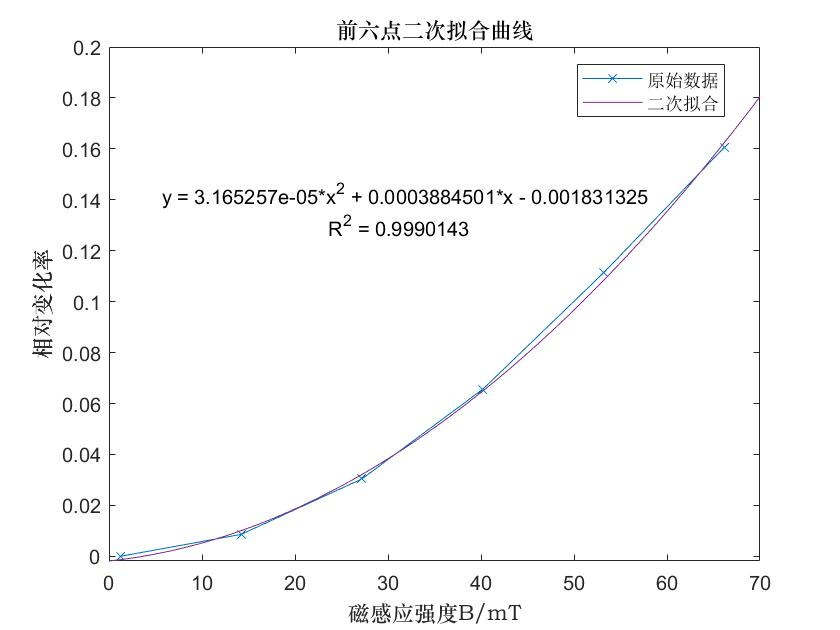
\includegraphics[width=0.9\linewidth]{拟合6.jpg}
	\end{minipage}
	%\qquad
	\begin{minipage}{0.49\linewidth}
		\centering
		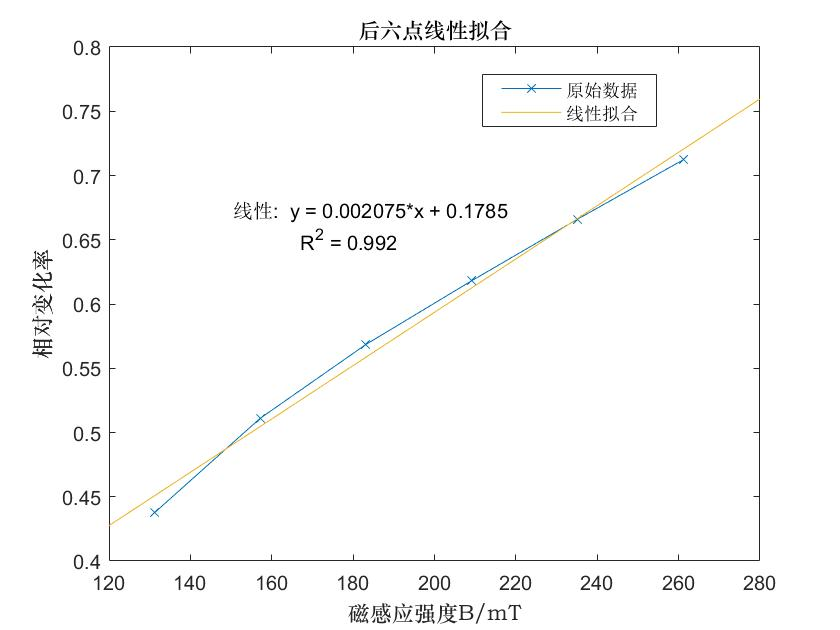
\includegraphics[width=0.9\linewidth]{拟合7.jpg}
	\end{minipage}
\end{figure}

根据实验讲义, 当  $0 \leq B \leq 60 m T$  时,  $\Delta R / R(0) \propto B^{2} $, 大致对应上图中前 6 个数据点, 符合二次函 数关系曲线; 当  $B \geq 120 m T$  时,  $\Delta R / R(0) \propto B$ , 大致对应上图中后 6 个数据点, 符合一次函数关系曲线。 对上述数据进行拟合, 计算得前 6 个点的相关系数  $R_{2}=0.9990$ , 二次函数关系理想; 后 6 个点的相关系数 $ R_{2}=0.992$ , 线性关系理想, 实验结果与理论分析相符。


\section{实验小结}

本次实验随测量数据较多,但原理并不复杂,且各组测量之间设计巧妙,相互关联,在认真预习的基础上,实验过程较为顺利,且有很多收获:

1.对霍尔效应有了新的认知。 高中阶段霍尔效应的内容,是基于载流子按平均速度运动的模型导出的,且不涉及各副效应影响。本次实验使我了解到载流子在霍尔元件中存在速度差异,且由于热流等因素会影响霍尔片输出电压,需要对理论模型和实验测量进行修正。认识到了实际物理体系的复杂性。

2.学习消除副效应的方法。 实验中,若待测量上叠加一系统误差,在改变实验条件时,误差与待测量大小不变而符号改变,且遵循不同的变化规律。可在改变实验条件时测量多组待测量,通过加减平均,保留待测量而抵消系统误差的影响;

3.设计合理的实验过程。 本实验需要改变 B、 I 的方向。 由于通过励磁电流 IM 换向改变 B的方向时, 由于电流较大,加上线圈电感效应的影响,容易产生电火花,因此应先对工作电流I换向, 再对 $I_M$ 换向, 最后再对 I 换向。

最后,感谢老师的悉心指导!



\section{实验原始数据}

\begin{figure}[H]
  \centering
  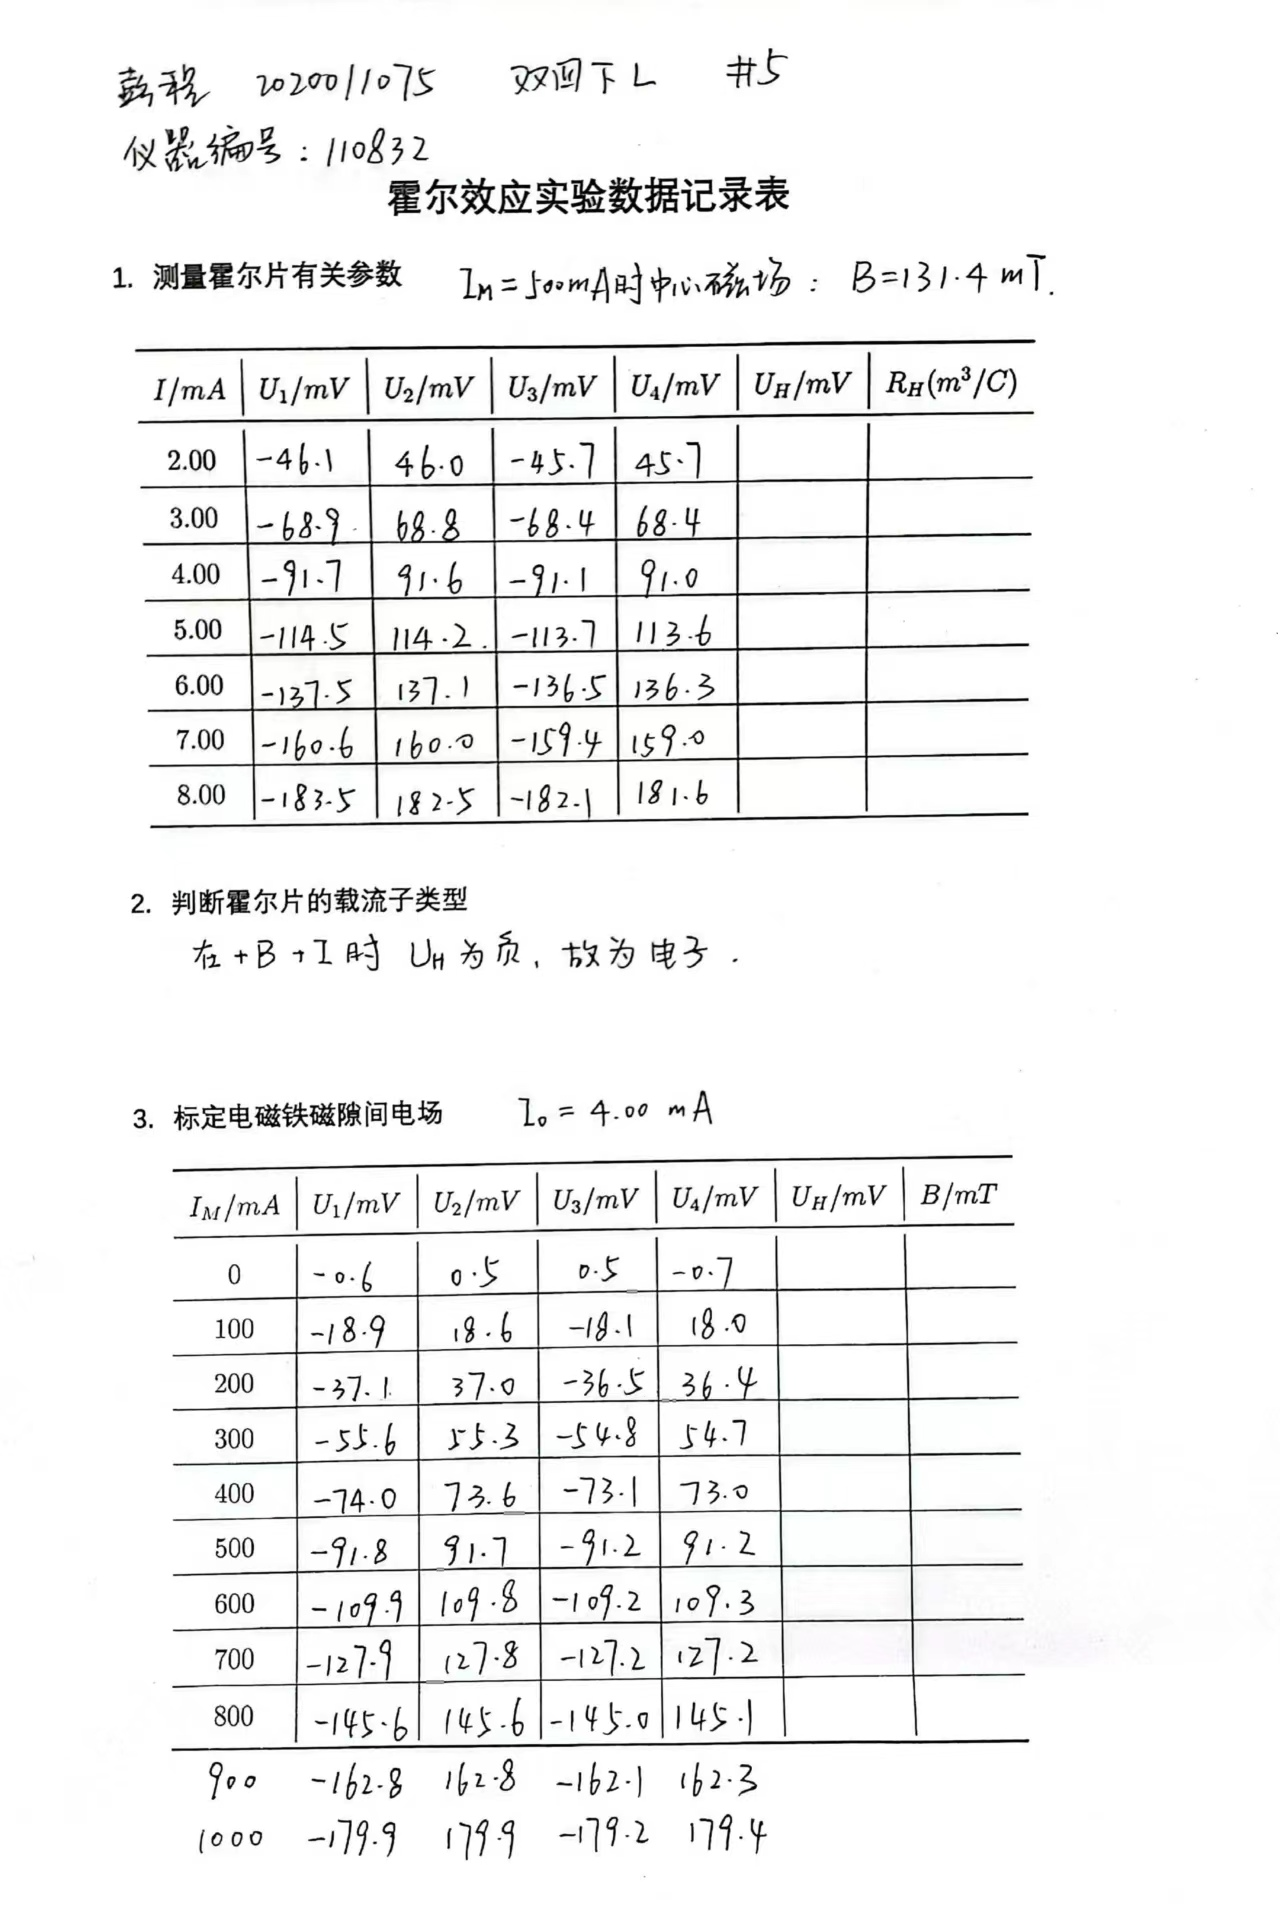
\includegraphics[scale=0.3]{记录1.jpg}
\end{figure}

\begin{figure}[H]
  \centering
  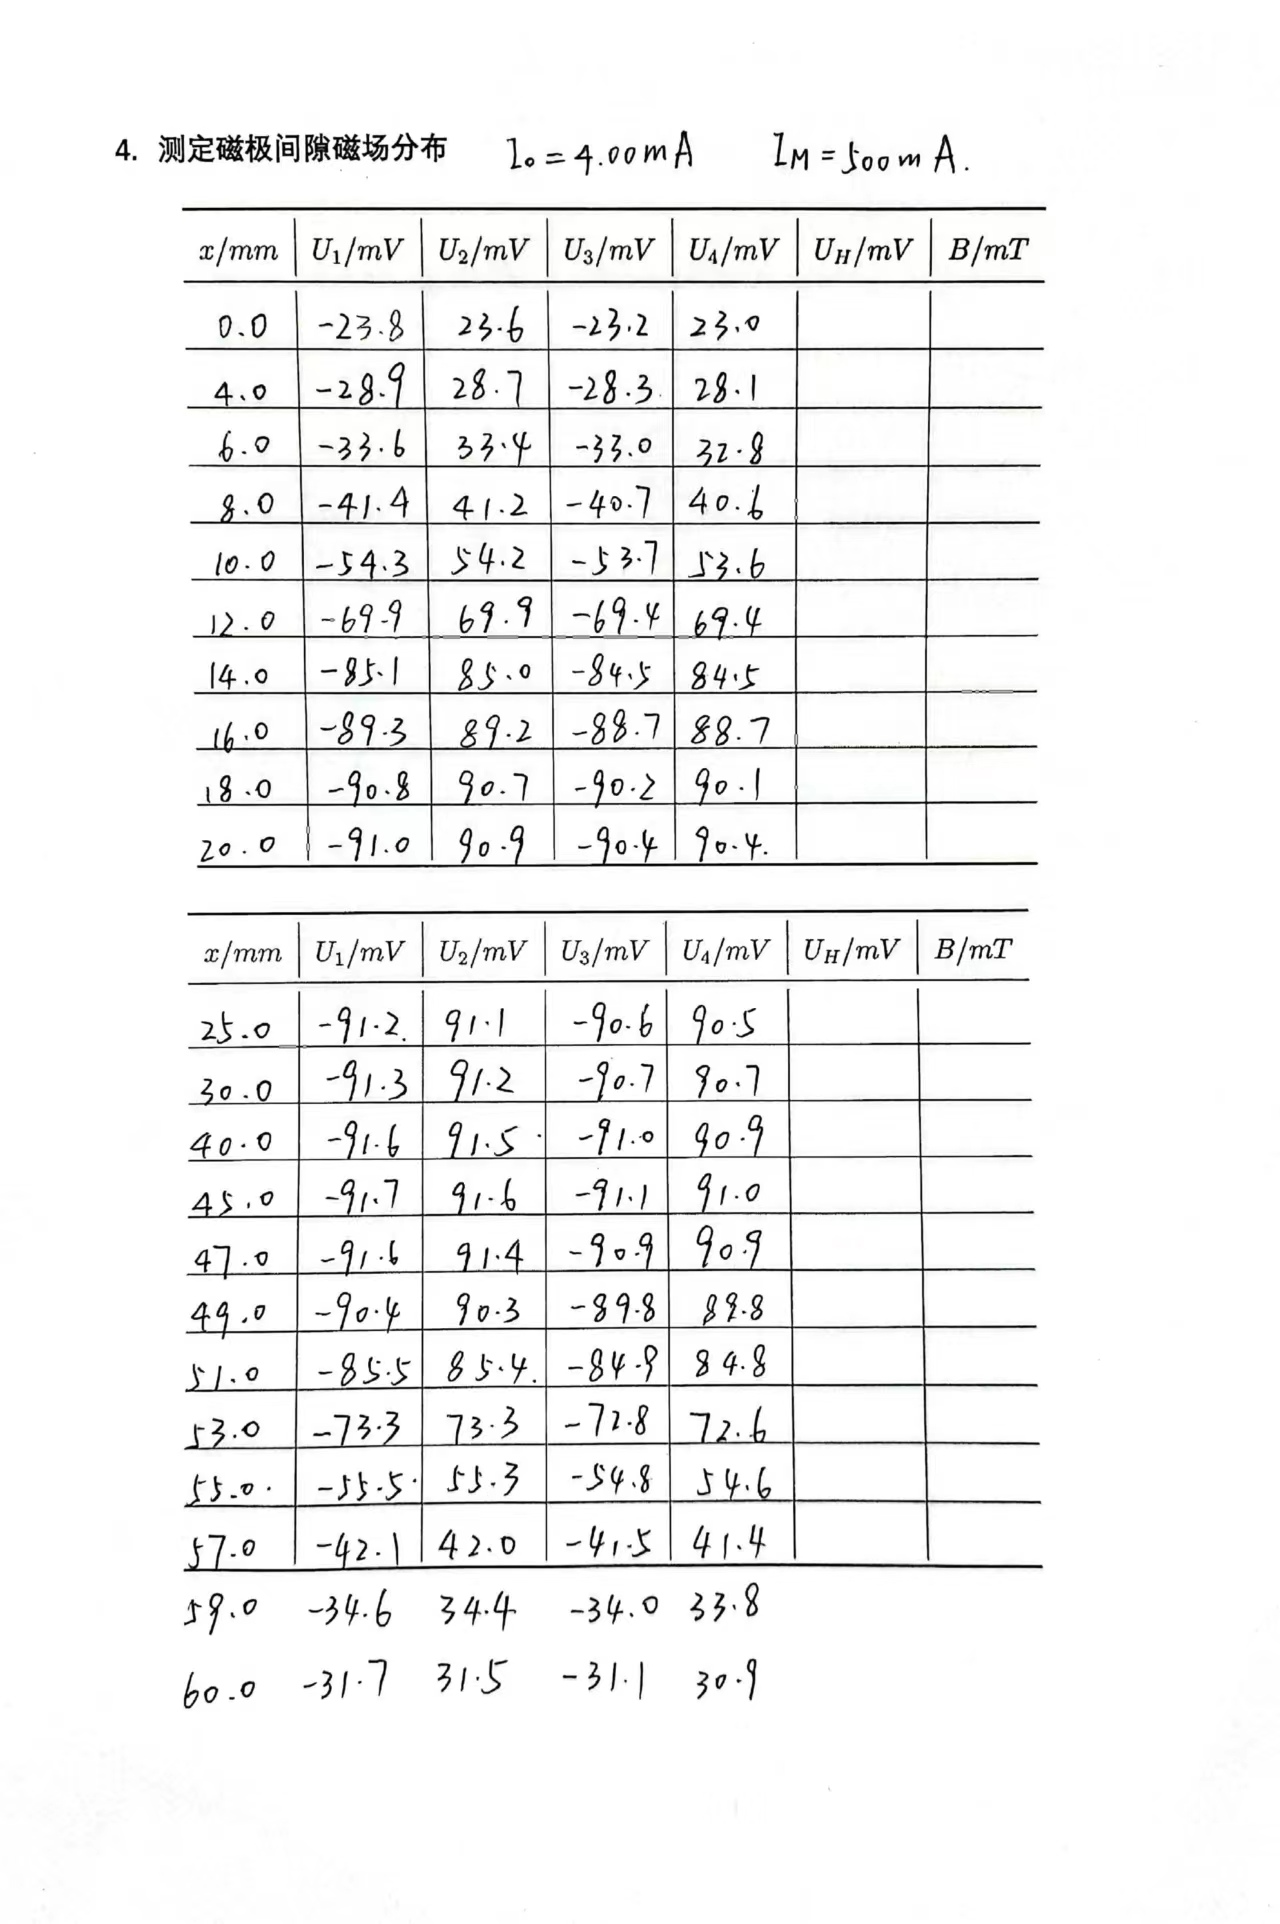
\includegraphics[scale=0.35]{记录2.jpg}
\end{figure}

\begin{figure}[H]
  \centering
  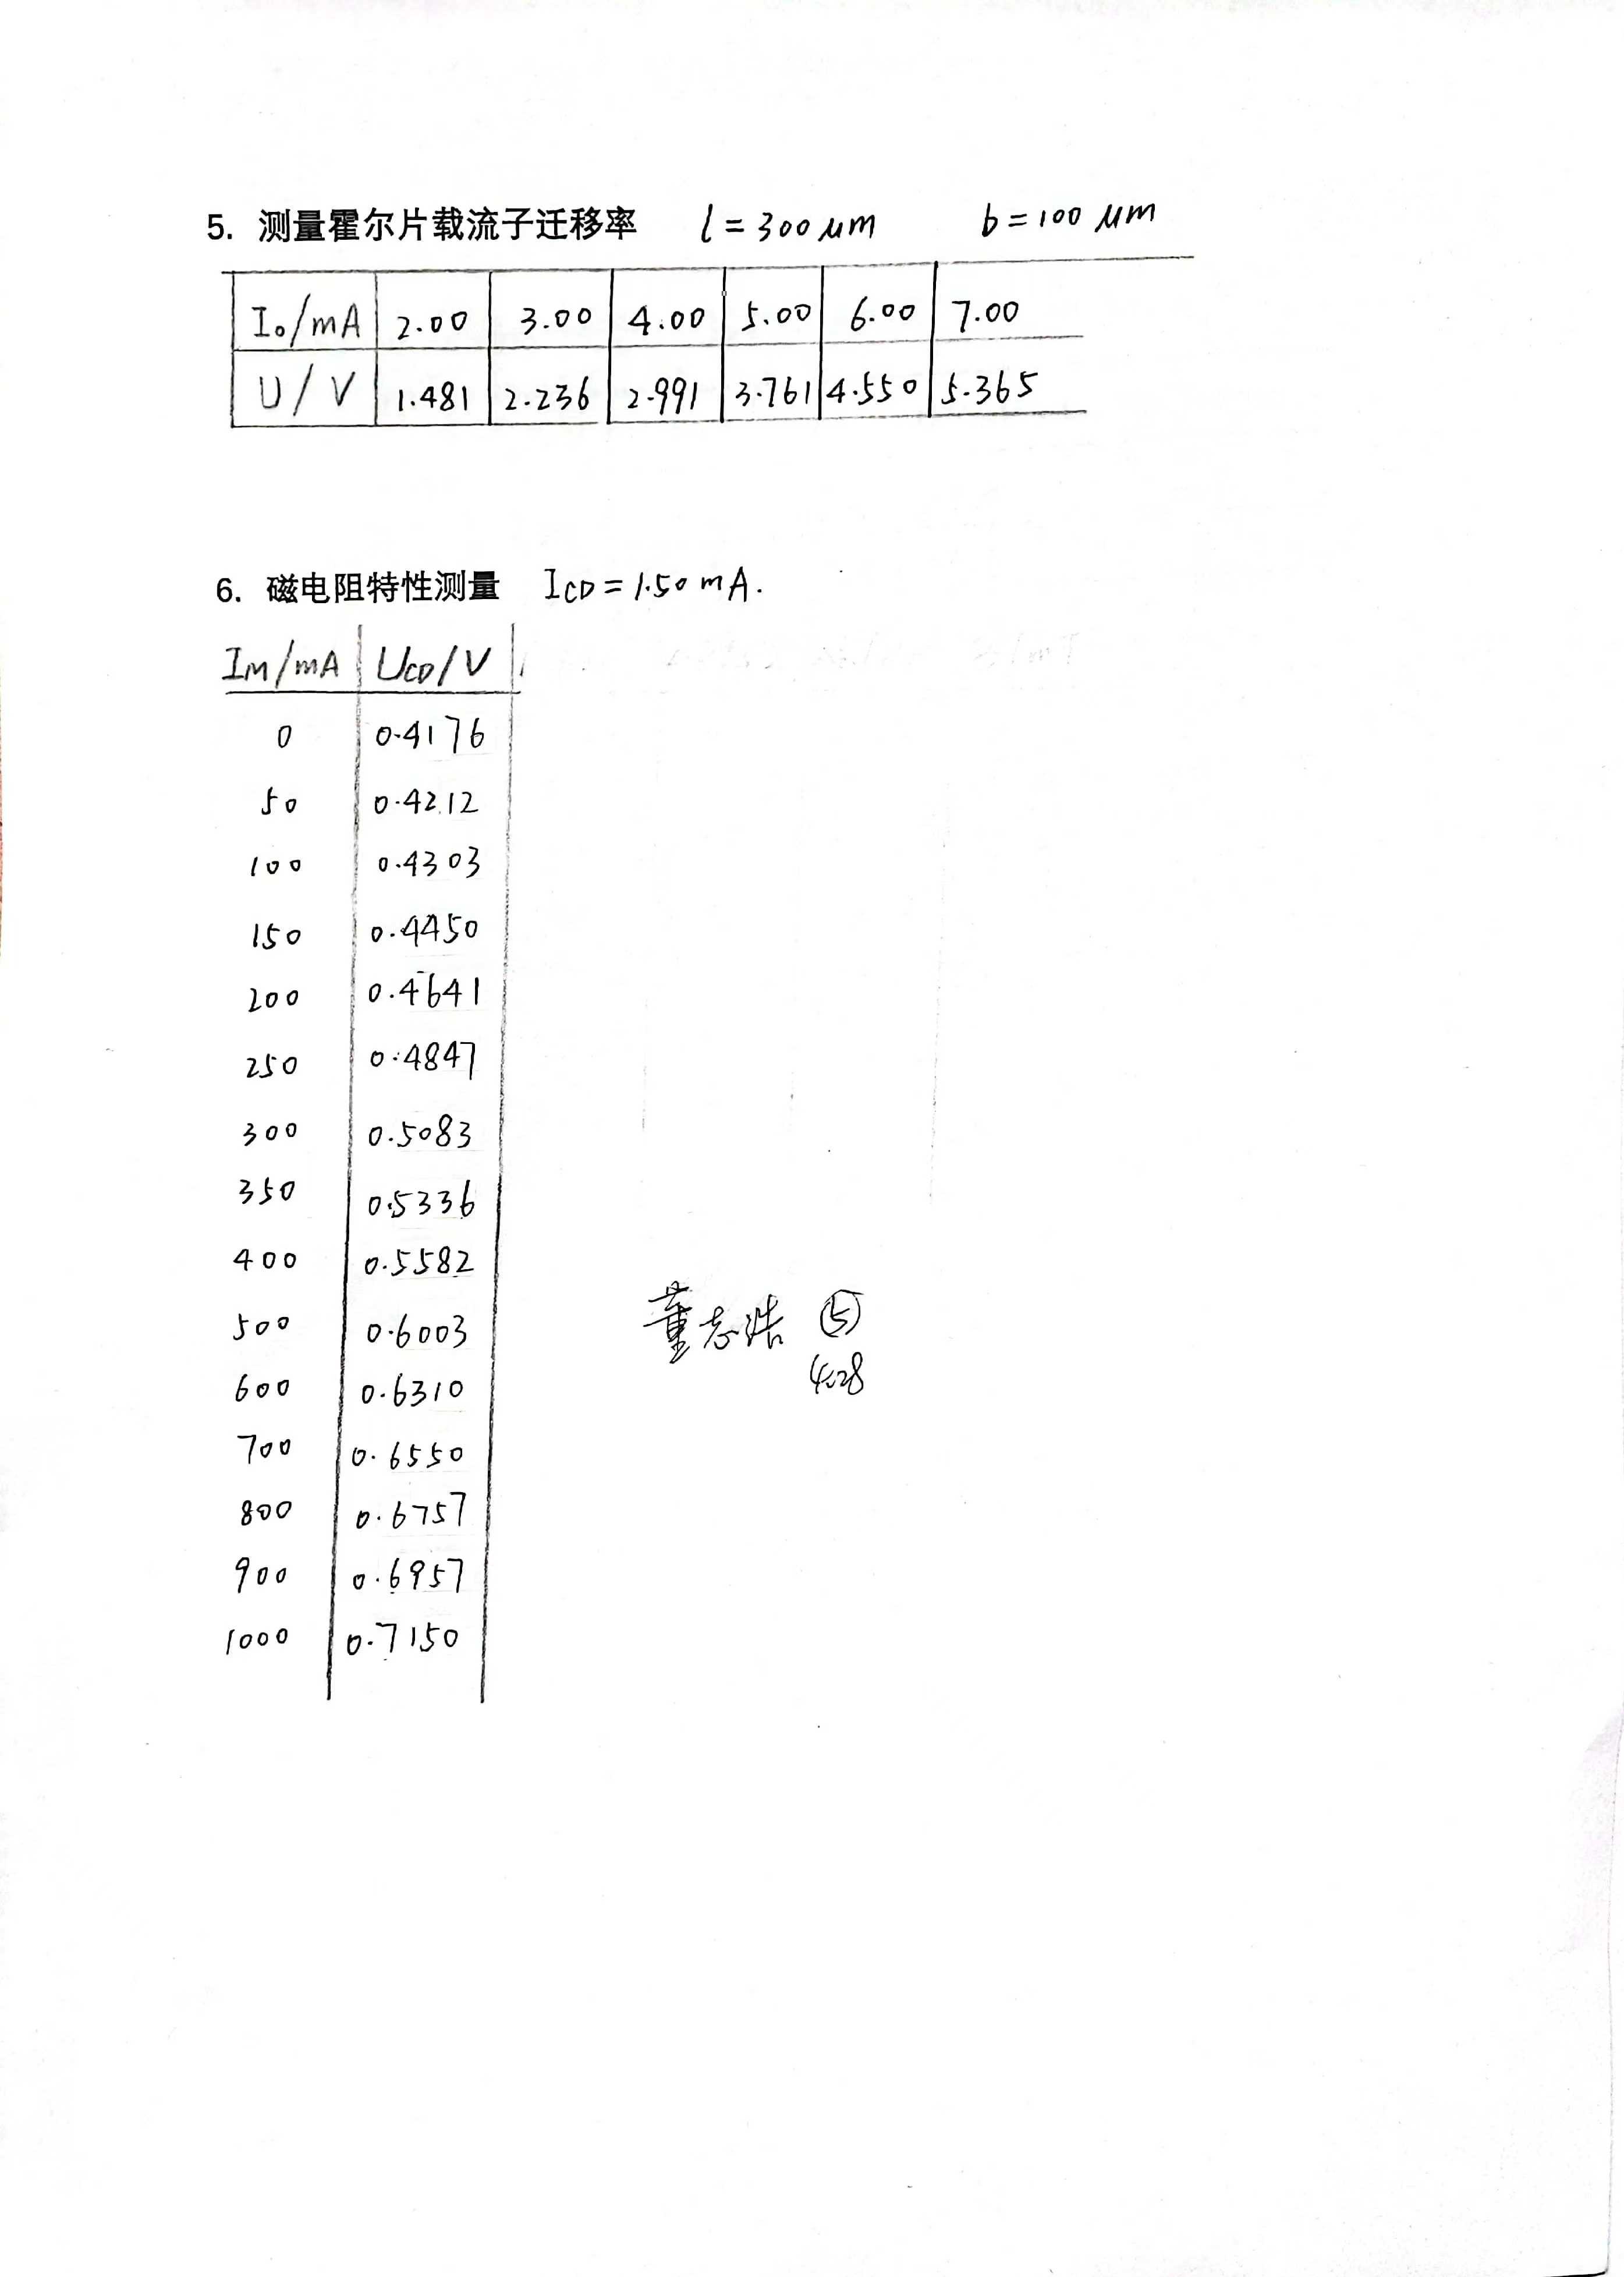
\includegraphics[scale=0.15]{记录3.jpg}
\end{figure}





\end{document}